% Automatically generated figure inventory for task1.

\begin{figure}[H]
\centering
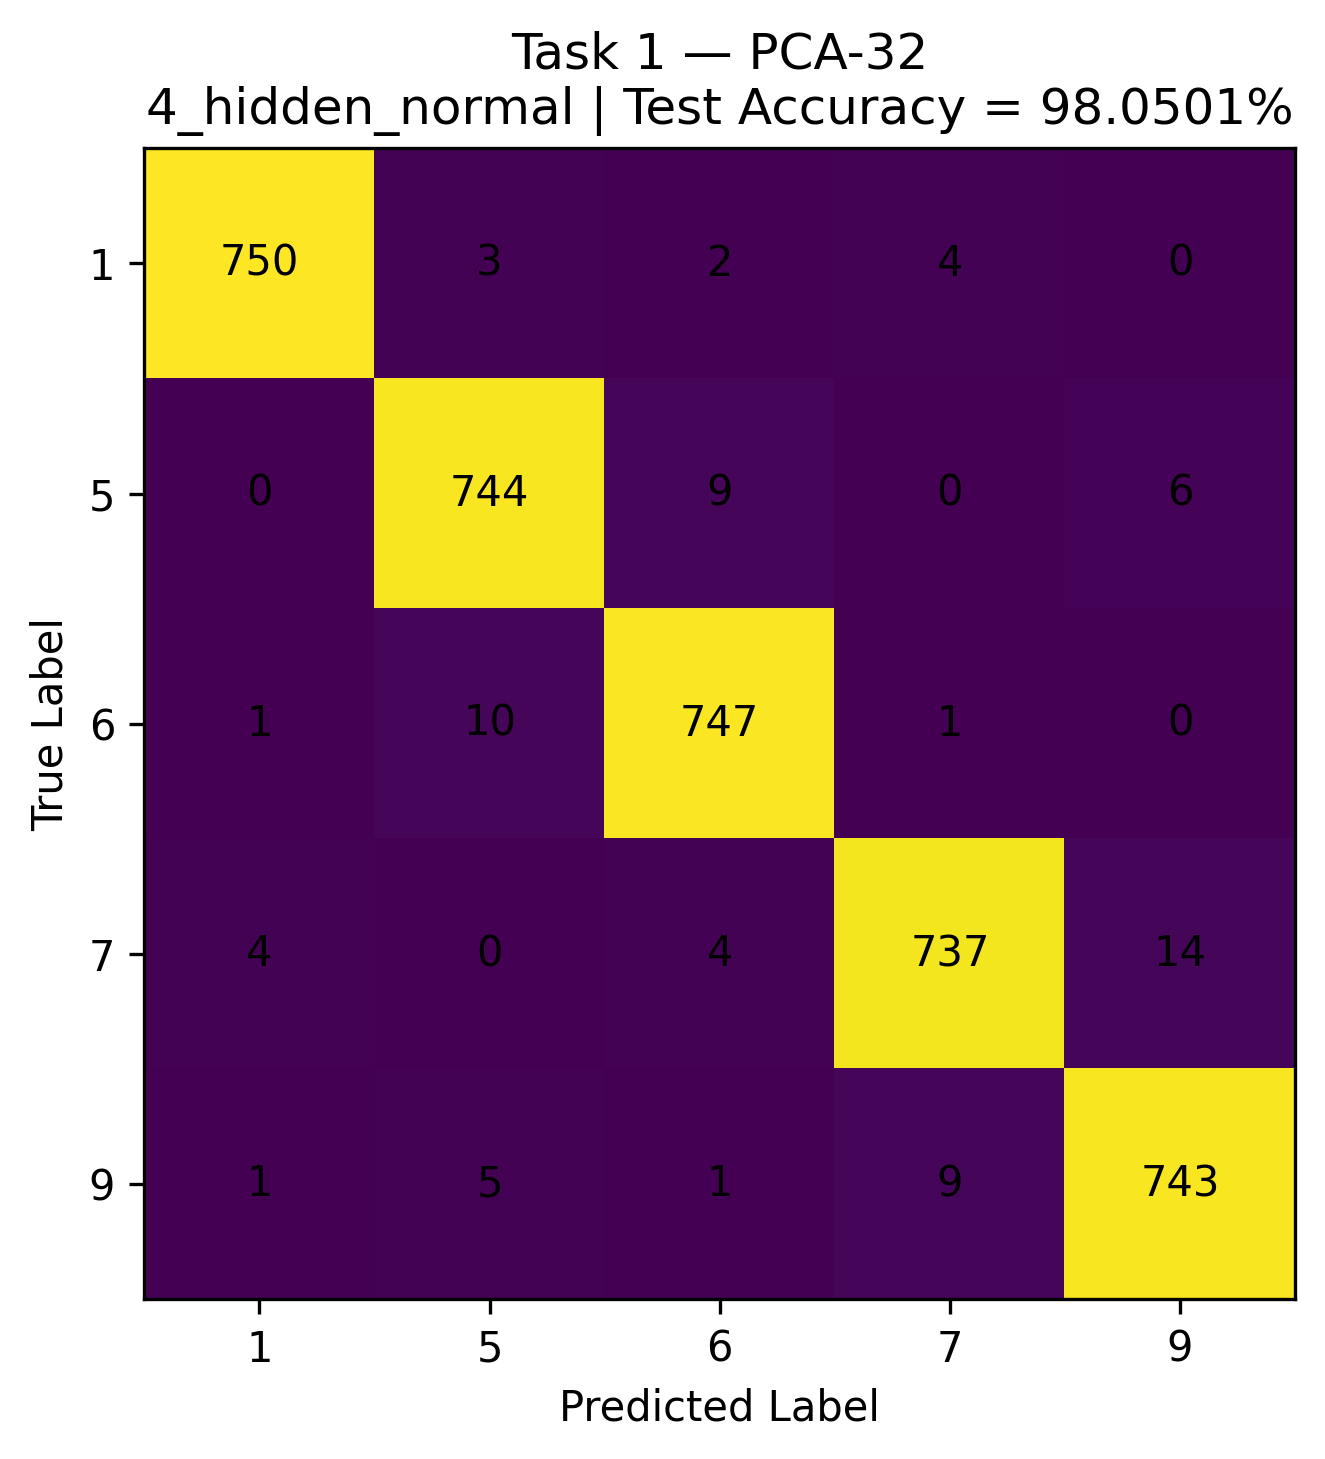
\includegraphics[width=0.88\linewidth,height=0.34\textheight,keepaspectratio]{figures/task1/cnf_mat_img/confusion_matrix_pca_32.png}
\caption{Confusion matrix: confusion matrix pca for 32 components.}
\label{fig:task1_1}
\end{figure}

\begin{figure}[H]
\centering
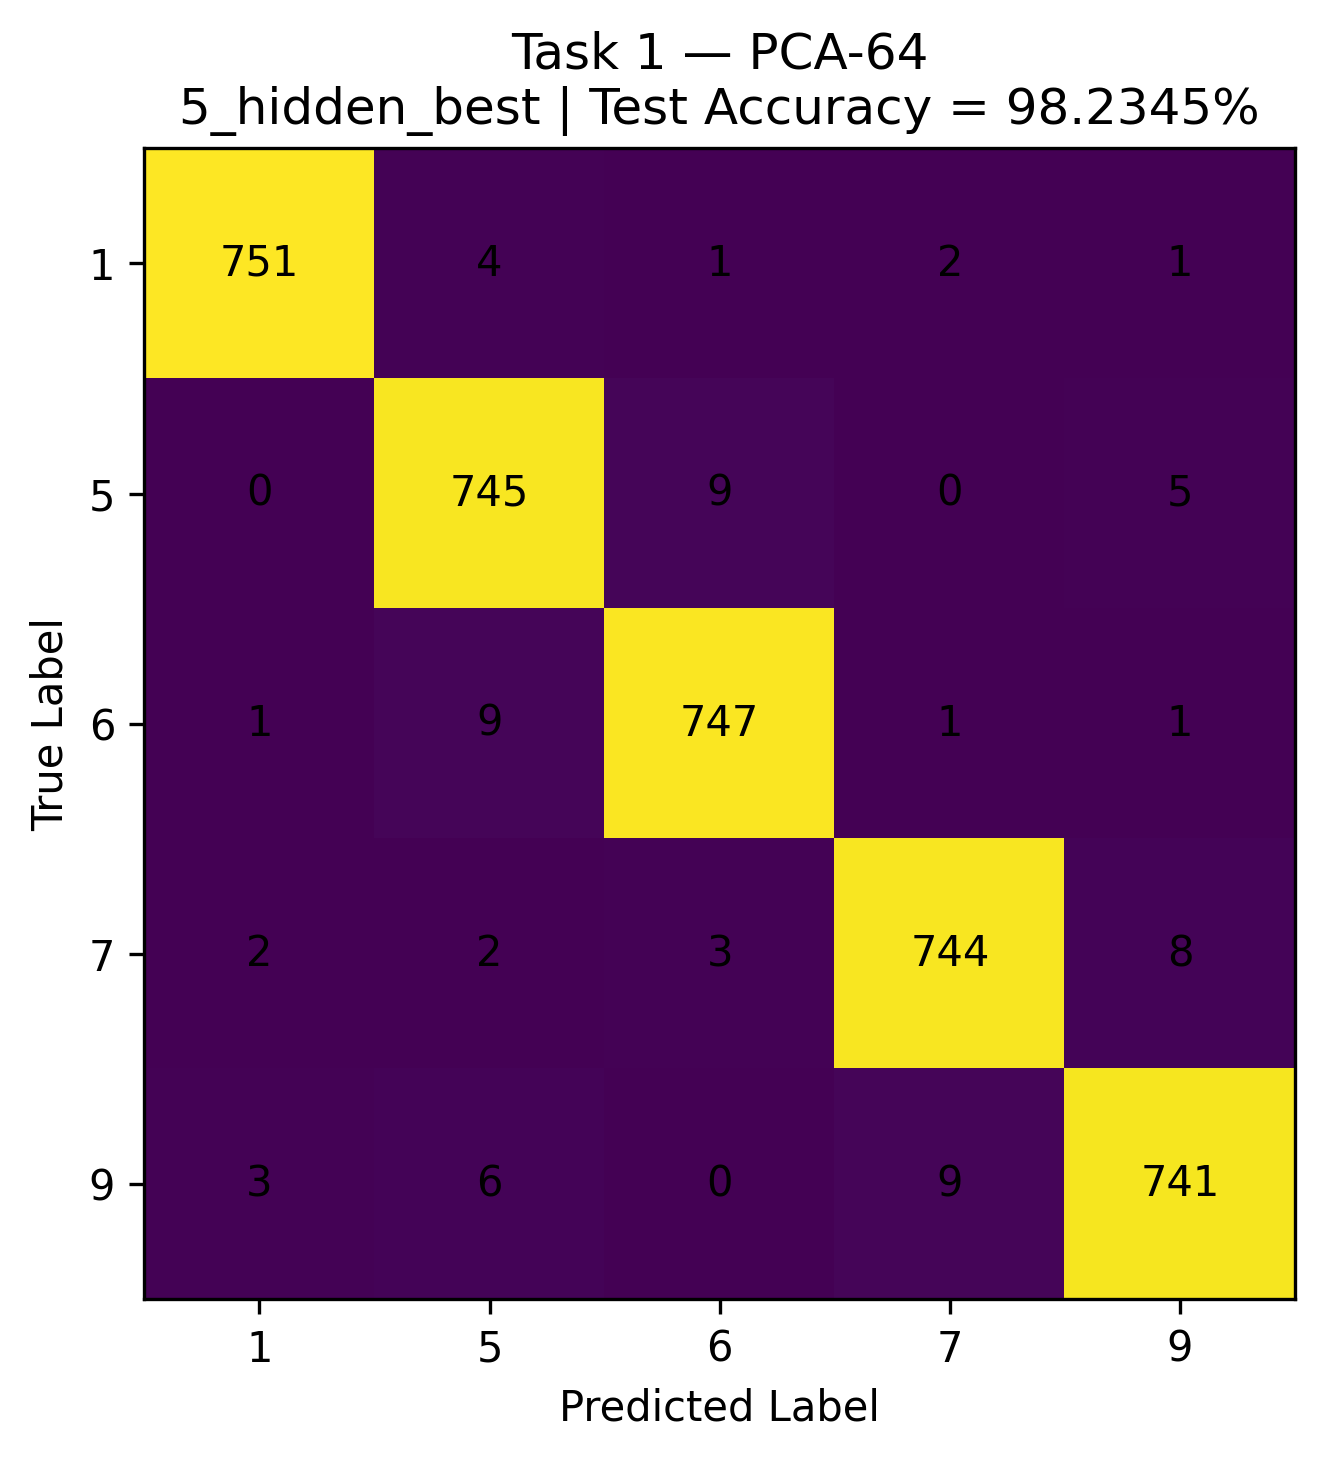
\includegraphics[width=0.88\linewidth,height=0.34\textheight,keepaspectratio]{figures/task1/cnf_mat_img/confusion_matrix_pca_64.png}
\caption{Confusion matrix: confusion matrix pca for 64 components.}
\label{fig:task1_2}
\end{figure}

\begin{figure}[H]
\centering
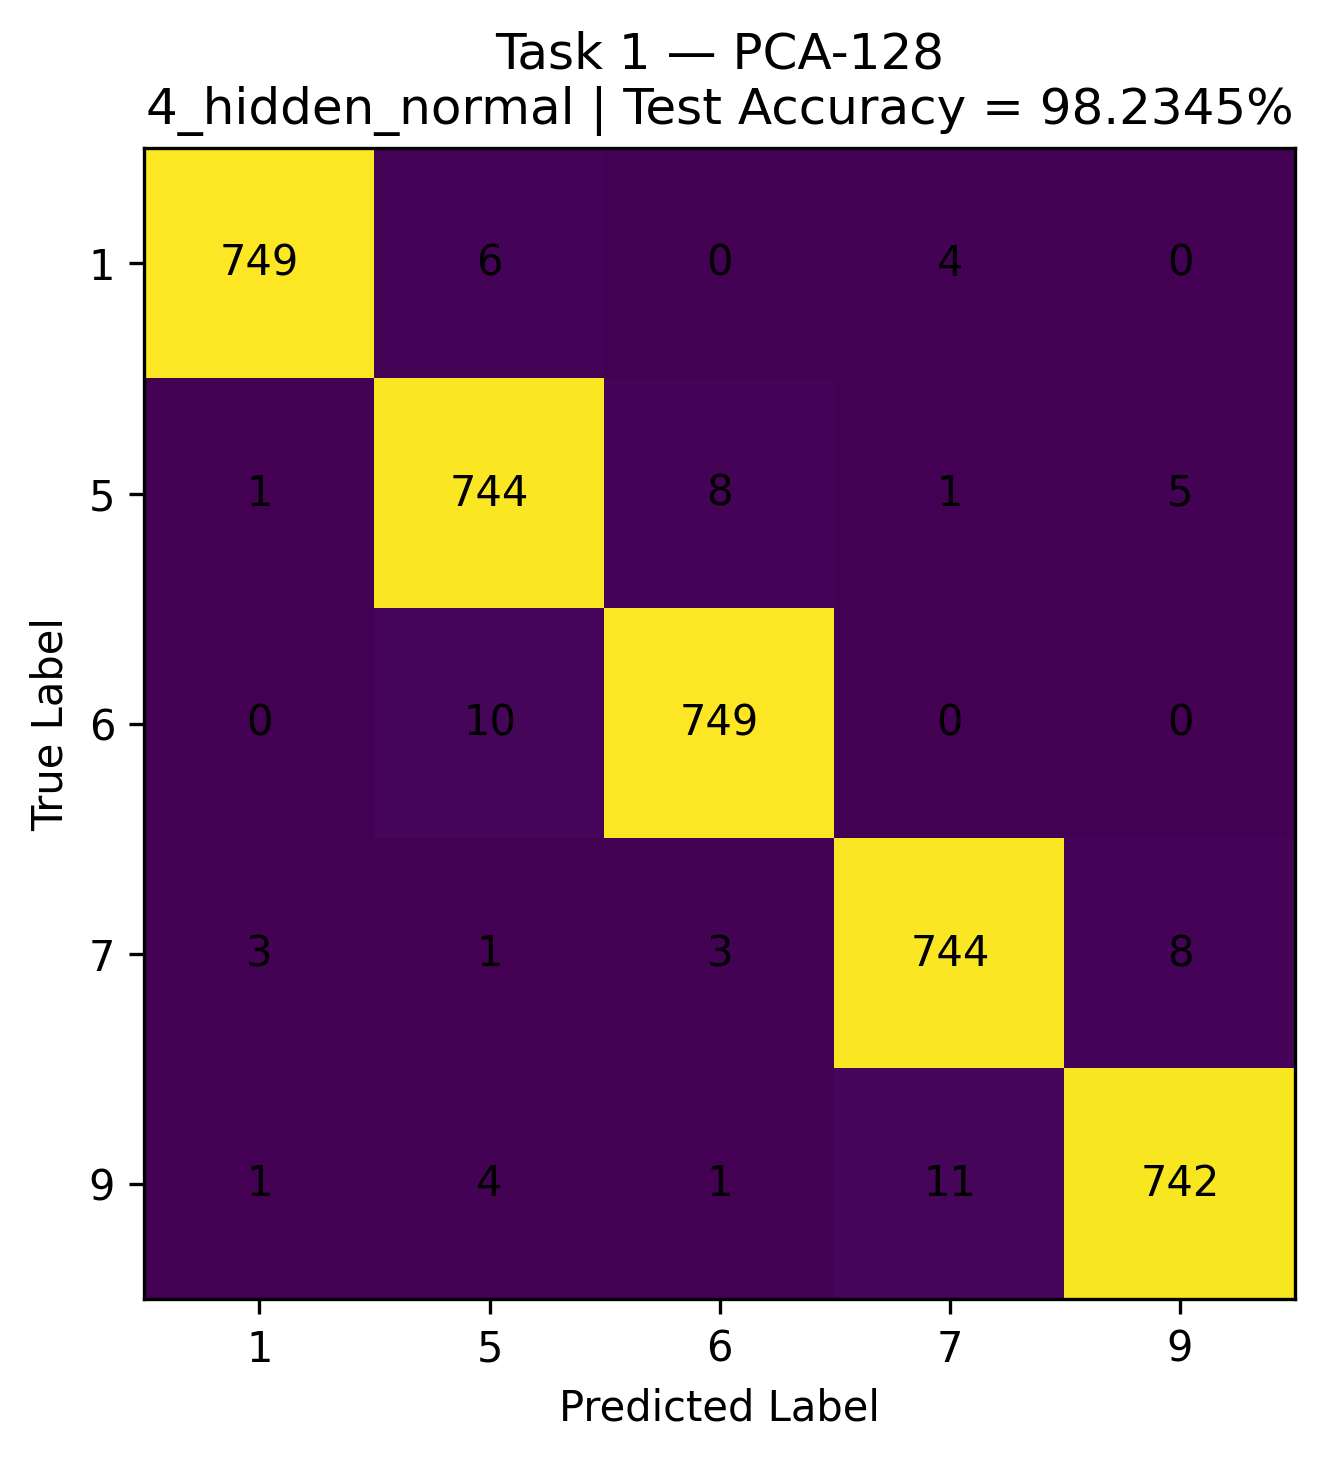
\includegraphics[width=0.88\linewidth,height=0.34\textheight,keepaspectratio]{figures/task1/cnf_mat_img/confusion_matrix_pca_128.png}
\caption{Confusion matrix: confusion matrix pca for 128 components.}
\label{fig:task1_3}
\end{figure}

\begin{figure}[H]
\centering
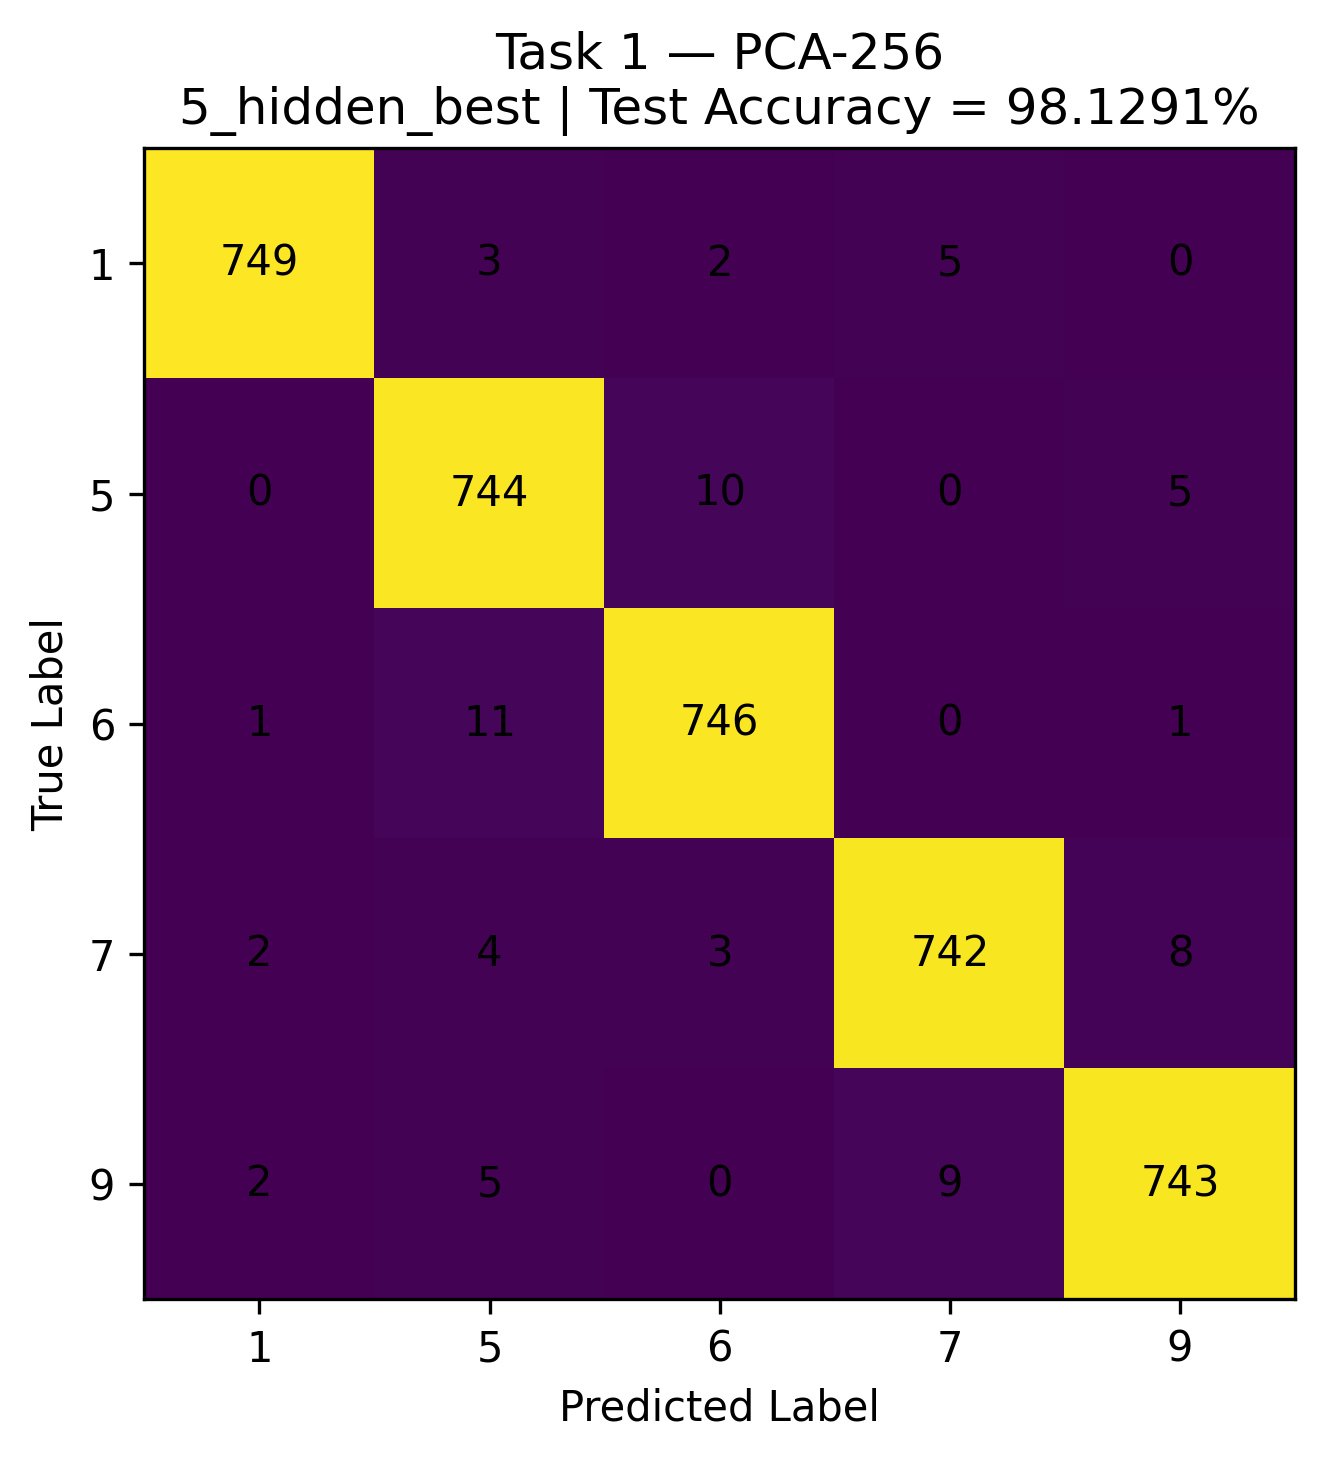
\includegraphics[width=0.88\linewidth,height=0.34\textheight,keepaspectratio]{figures/task1/cnf_mat_img/confusion_matrix_pca_256.png}
\caption{Confusion matrix: confusion matrix pca for 256 components.}
\label{fig:task1_4}
\end{figure}
